\documentclass[11pt,a4paper]{article}
\usepackage[T1]{fontenc}
%\usepackage[latin1]{inputenc}
%\usepackage{amssymb,amsmath,a4wide}
\usepackage[utf8]{inputenc}
\usepackage{amssymb,amsmath}
\usepackage{nicefrac}
\usepackage[pdftex]{graphicx}
\usepackage{ctable}
\usepackage{amsmath}
%\usepackage{threeparttable} %na
%\usepackage{tabu} %na
\usepackage{tabularx}
\usepackage{subfig}
\usepackage{rotating}
\usepackage{longtable}
%\usepackage[table]{xcolor} % clash with floatrow
\usepackage{xcolor} 
\usepackage{threeparttable}
%\usepackage[multiple]{footmisc} %na
\usepackage{bm}
\usepackage{fancybox}
%\usepackage{harvard}
\usepackage{geometry}         % Definir les marges
\geometry{verbose,a4paper,tmargin=1in,bmargin=1in,lmargin=1in,rmargin=1in}
\usepackage{setspace}
%\usepackage{ccaption}
\usepackage[colorlinks=true,citecolor=black, urlcolor=black, linkcolor=black]{hyperref}
\usepackage{url}
\newcommand{\email}[1]{\href{mailto:#1}{\nolinkurl{#1}}}
%\usepackage[longnamesfirst]{natbib}
\usepackage{natbib}
\usepackage[french, english]{babel}  % Placez ici une liste de langues, la derniere etant la langue principale
\usepackage{caption}
\usepackage{floatrow}
\usepackage{lscape}
\usepackage{afterpage}
\usepackage{supertabular}    %na            %  mettre pour les grands tableaux en formant paysage. marche avec \begin{landscape}
% style de la biblio : necessaire pour utiliser BibTex, necessite le deuxieme fichier exemple.bib


\bibliographystyle{elsarticle-harv}
\newcommand{\tqdl}{\textquotedblleft}
\newcommand{\tqdr}{\textquotedblright}
\linespread{1.2}

\begin{document}
\title{Answers to Hubert Escaith\\
\vspace{1cm}
}
\vspace{1cm}
\date{\today}
\author{Guillaume Daudin\thanks{PSL, Universit\'e Paris-Dauphine,Sciences Po, OFCE. E-mail: \email{guillaume.daudin@dauphine.psl.eu}}}
%\vspace*{\fill}
\maketitle

\section{Why not based on VA trade ?}
Why don't we simply : \\
1. Compute the origin of the VA content of each good \\
2. Study how the price evolve following a shock on the price of VA in a country or another ?

Intuition: \\
That would not do because the price of, e.g. French VA does not change for everybody.

Doubt: is that enough an argument ?
1 sector, 2 countries
\subsection{Evolution of VA price}
\begin{gather*}
A=\left(\begin{matrix}a_{1,1}&a_{1,2}\\a_{2,1}&a_{2,2}\end{matrix}\right)
\\
I-A=\left(\begin{matrix}1-a_{1,1}&-a_{1,2}\\-a_{2,1}&1-a_{2,2}\end{matrix}\right)
\\
\left(I-A\right)^{-1}=\frac{1}{\left(1-a_{1,1}\right)\left(1-a_{2,2}\right)-a_{2,1}a_{1,2}}\left(\begin{matrix}1-a_{2,2}&a_{1,2}\\a_{2,1}&1-a_{1,1}\end{matrix}\right) =z.\left(\begin{matrix}1-a_{2,2}&a_{1,2}\\a_{2,1}&1-a_{1,1}\end{matrix}\right) \\ 
=\left(\begin{matrix}u&v\\w&x\end{matrix}\right)
\\
\text{French demand shares}=d=\left(\begin{matrix}1-f\\f\end{matrix}\right) \\
\left(I-A\right)^{-1}d=\left(\begin{matrix}u-uf+vf\\w-wf+xf\end{matrix}\right)
\end{gather*}

Donc, en cas de choc $c$ pour le prix de la va dans le pays étranger (en monnaie française), on peut écrire un vecteur de choc : $C=\left(0,c\right)$.  les prix varient tout d'abord de  $CA$, puis $CA^2$, etc. Donc le vecteur de choc $S$ (en monnaie française) est : 


\begin{equation*}
S=C+CA+CA^2...=C(I-A)^{-1}=\left(\begin{matrix}cw  &   cx\end{matrix}\right)
\end{equation*}

To measure the effect on French consumption prices, we do a weighted sum of these effects.

\begin{equation}
\bar{s}=c.\left[\left(1-f\right)w+xf\right]=c.\frac{\left(1-f\right)a_{2,1}+f\left(1-a_{1,1}\right)}{\left(1-a_{1,1}\right)\left(1-a_{2,2}\right)-a_{2,1}a_{1,2}}
\end{equation}

If each nation's production only uses national inputs, we have a plausible :
\begin{equation*}
\bar{s}=c.\frac{f}{1-a_{2,2}}
\end{equation*}

\subsection{Exchange rate shock}

Using the notations in the paper...

\begin{gather*}
C=\left(0,\frac{-c_\$}{1+c_\$}\right)=\left(0,-c\right)
\\
C_\$=\left(c_\$,0\right)
\\
\tilde{C}_\$=\left(0,-c_\$\right)
\\
\hat{C}_\$=\left(\frac{c_\$}{1+c_\$},0\right)=\left(c,0\right)
\\
\cal B = \left(\begin{matrix}0&a_{1,2}\\0&0\end{matrix}\right)
\\
\tilde{\cal B} = \left(\begin{matrix}0&0\\a_{2,1}&0\end{matrix}\right)
\end{gather*}

Hence

\begin{gather*}
S =\left(0,c\right)+\left[\left(0,-c.a_{1,2}\right)+\left(c.a_{2,1},0\right)\right]*\left(\begin{matrix}u&v\\w&x\end{matrix}\right)
\\
=\left(0,c\right)+\left(c.a_{2,1},-c.a_{1,2}\right)*\left(\begin{matrix}u&v\\w&x\end{matrix}\right)
\\
=\left(0,c\right)+\left(u.c.a_{2,1}-w.c.a_{1,2},v.c.a_{2,1}-x.c.a_{1,2}\right)
\\
=\left(u.c.a_{2,1}-w.c.a_{1,2},c+v.c.a_{2,1}-x.c.a_{1,2}\right)
\end{gather*}
and
\begin{gather*}
\bar{s}=\left(u.c.a_{2,1}-w.c.a_{1,2},c+v.c.a_{2,1}-x.c.a_{1,2}\right).\left(\begin{matrix}1-f\\f\end{matrix}\right)
\\
\bar{s}=c\left[f\left(1+v.a_{2,1}-x.a_{1,2}\right)+\left(1-f\right)\left(u.a_{2,1}-w.a_{1,2}\right)\right]
\end{gather*}


If each nation's production only uses national inputs, we have a plausible

\begin{gather*}
\bar{s}=c.f
\end{gather*}

This seems to confirm that the exchange rate shock is not the same as the VA price shock.

\section{Residual issue}
\subsection{Presenting the issue}

As a reminder from the paper, where $\overline{s}_{i}^{i,HC}$ is the effect of an exchange rate shock on consumption prices :  
\begin{equation}
\begin{array}{lccl}
\overline{s}_{i}^{i,HC}&=S^i.HC^i=E1.HC^i+E2.HC^i+E3.HC^i+E4.HC^i \\
&=E1.HC^{i,imp}+E2.HC^{i,dom}+E3.HC^{i,imp}+E4.HC^i
 \end{array} 
 \end{equation}
 
 and

\begin{equation}
\begin{array}{lccl}
	S^ i&=&C^i	&+ \left(\hat{C}^i_\$.{\cal B}+{C^i}{\tilde{{\cal B}}}\right)*{{(I-{\cal A})}^{-1}} \\
	S^i &=&\underbrace{C^i}_{\substack{\text{(E1) direct effect through} \\ \text{ imported consumption goods}}}&+ \underbrace{{C^i}{\tilde{{\cal B}}}}_{\substack{\text{(E2) effect on} \\ \text{ \emph{domestic} consumption goods} \\ \text{ through \emph{imported} inputs}}}  + \underbrace{\hat{C}^i_\$.{\cal B}}_{\substack{\text{(E3)  effect on} \\ \text{\emph{imported} consumption goods} \\ \text{through \emph{domestic} inputs}}} \\ &&+\underbrace {\left( \hat{C}^i_\$.{\cal B} + {C^i}{\tilde{{\cal B}}}\right)*{{(I-{\cal A})}^{-1}}*{\cal A}}_{\text{(E4) residual}} \\
\end{array}
\end{equation}



When the shock corresponds to an appreciation of the domestic currency, $E1$ and $E2$ reduce country $i$'s household consumption prices and $E3$ increases country $i$'s household consumption prices. Notice that $E1$ and $E2$ are easy to compute with national input-output matrices, whereas world input-output matrices are needed for computing $E3$ and $E4$.

We have the strange result that $E3 + E4$ seems to be constant, whatever the openness rate of the economy (see Figure \ref{fig:ratiodir_WIOD})

\begin{figure}[!h]
\centering
\caption{\footnotesize{\textbf{Comparing $\overline{s}_{i}^{i,HC}$ and $E1.HC^{i,imp}+E2.HC^{i,dom}$}}}
\begin{tabular}{c}
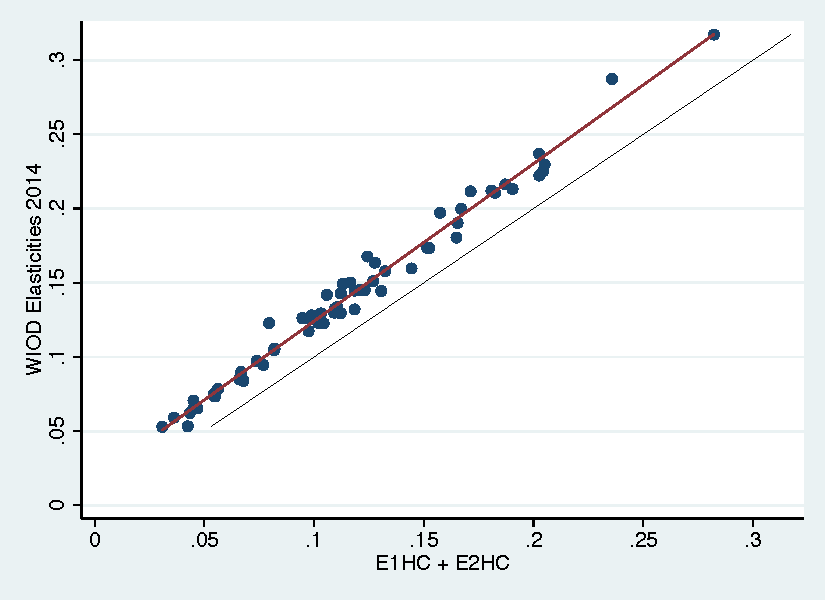
\includegraphics[width=5.0in, height=3.5in]{graph_2014_WIOD_HC}\\
\end{tabular}
\label{fig:ratiodir_WIOD}
\end{figure}

Let us see what happens in a 2 country, 1 sector economy : 

\begin{gather*}
E1=C=\left(0,-c\right)
\\
E2=C.\tilde{\cal B}=\left(0,-c\right).\left(\begin{matrix}0&0\\a_{2,1}&0\end{matrix}\right)=\left(-c.a_{2,1},0\right)
\\
E3=(c,0).\left(\begin{matrix}0&a_{1,2}\\0&0\end{matrix}\right)=\left(0,c.a_{1,2}\right)
\end{gather*}

\begin{gather*}
E1.HC = \left(0,-c\right).\left(\begin{matrix}1-f\\f\end{matrix}\right)=-f.c
\\
E2.HC=\left(-c.a_{2,1},0\right).\left(\begin{matrix}1-f\\f\end{matrix}\right)=-c.a_{2,1}.\left(1-f\right)
\\ 
E3.HC=\left(0,c.a_{1,2}\right).\left(\begin{matrix}1-f\\f\end{matrix}\right)=f.c.a_{1,2}
\end{gather*}

We do not loose any generality by normalizing the shock $c$ to 1. 

And, developped from SAGE :
\begin{gather}
\bar{s}-E1.HC-E2.HC=\left(\begin{array}{r}
-\frac{a_{12} a_{21}^{2} - a_{11} a_{21} a_{22} + {\left(a_{11} - a_{12}\right)} a_{21} - {\left(a_{12} a_{21}^{2} - a_{11} a_{21} a_{22} - {\left(a_{11} - 1\right)} a_{12} + {\left(a_{11} - 2 \, a_{12}\right)} a_{21}\right)} f}{a_{12} a_{21} - {\left(a_{11} - 1\right)} a_{22} + a_{11} - 1}
\end{array}\right)
\end{gather}

We had some hypothesis to check if we get something that we can study in its symbolic form:
$\frac{a_{1,1}}{a_{2,1}}=\frac{1-f}{f}$ and $a_{1,1}+a_{2,1}=a$. \\ 
So
$a_{1,1}=(1-f)a$ and $a_{2,1}=fa$.
Then:

\begin{gather}
residual=\left(\begin{array}{r}
-\frac{{\left(a^{2} a_{12} + a^{2} a_{22} - a^{2}\right)} f^{3} - {\left(2 \, a^{2} a_{22} - 2 \, a^{2} + {\left(a^{2} + a\right)} a_{12}\right)} f^{2} + {\left(a^{2} a_{22} - a^{2} + a_{12}\right)} f}{{\left(a - 1\right)} a_{22} - {\left(a a_{12} + a a_{22} - a\right)} f - a + 1}
\end{array}\right)
\end{gather}

According to SAGE, the derivative of this according to f is: 
\begin{gather*}
\left(\begin{array}{r}
-\frac{{\left({\left(a^{2} a_{12} + a^{2} a_{22} - a^{2}\right)} f^{3} - {\left(2 \, a^{2} a_{22} - 2 \, a^{2} + {\left(a^{2} + a\right)} a_{12}\right)} f^{2} + {\left(a^{2} a_{22} - a^{2} + a_{12}\right)} f\right)} {\left(a a_{12} + a a_{22} - a\right)}}{{\left({\left(a - 1\right)} a_{22} - {\left(a a_{12} + a a_{22} - a\right)} f - a + 1\right)}^{2}} \\
- \frac{a^{2} a_{22} + 3 \, {\left(a^{2} a_{12} + a^{2} a_{22} - a^{2}\right)} f^{2} - a^{2} - 2 \, {\left(2 \, a^{2} a_{22} - 2 \, a^{2} + {\left(a^{2} + a\right)} a_{12}\right)} f + a_{12}}{{\left(a - 1\right)} a_{22} - {\left(a a_{12} + a a_{22} - a\right)} f - a + 1}
\end{array}\right)
\end{gather*}

I do not think we can do much with this. So we move to a numerical application.

\subsection{Numerical application}
From WIOD2014, I can compute the ration between VA and production. The computation with the WIOD data is : 
egen total=rowtotal(vAUS1-vROW) and then (161-74)/161=54\%.

For simplification, I assume that the ratio is equal to 0.5.
\begin{gather*}
a_{1,1}+a_{1,2}=a_{2,1}+a_{2,2}=50\% \\
\frac{a_{1,2}}{a_{1,1}+a_{1,2}}=f \\
a_{2,1}=0.48 \\
a_{2,2}=0.02
\end{gather*}
The excel file (2019 01 calcul matrice pour résidu) shows that the residual is not proportional to f.
Back to sage...
\begin{gather*}
\left(\begin{array}{r}
\frac{-0.125 \, f^{3} + 0.245 \, f^{2} - 0.11 \, f}{-0.25 \, f - 0.26
}
\end{array}\right)
\end{gather*}

Which yields Figures \ref{fig:resid} and \ref{fig:tous_les_E}.
\begin{figure}[!h]
\begin{center}
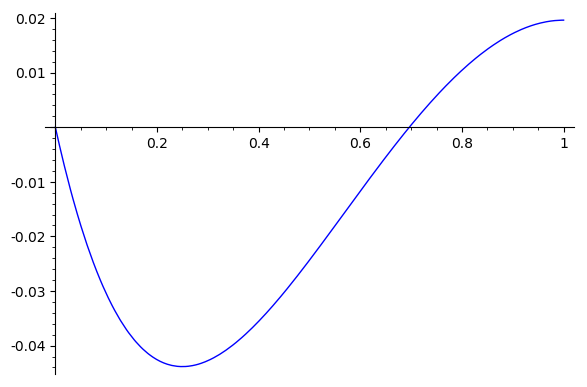
\includegraphics{etude_residu.png}
\caption{Residual as a function of the openness rate}
\label{fig:resid}
\end{center}
\end{figure}

The zone of interest is between 0.15 and 0.5. In that zone, the relationship between the openness rate and the residual is not monotonous, and actually does not vary much (see Figure \ref{fig:resid}).

and
\begin{figure}[!h]
\begin{center}
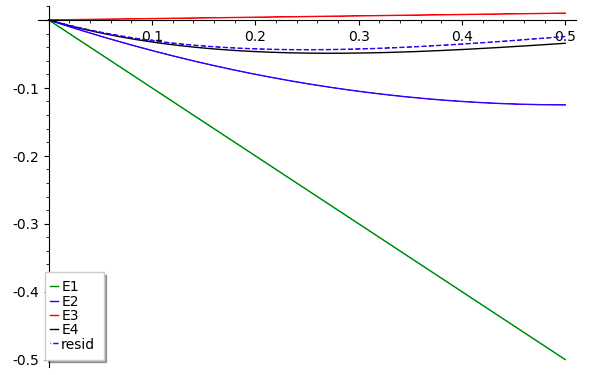
\includegraphics{etude_tous_les_E.png}
\caption{All the Es plus the residual}
\label{fig:tous_les_E}
\end{center}
\end{figure}


\end{document}